% Copyright (c) 2017 Ongun Kanat <ongun.kanat@gmail.com>
% Permission is hereby granted, free of charge, to any person obtaining a copy of 
% this software and associated documentation files (the "Software"), to deal in 
% the Software without restriction, including without limitation the rights to 
% use, copy, modify, merge, publish, distribute, sublicense, and/or sell copies of 
% the Software, and to permit persons to whom the Software is furnished to do so, 
% subject to the following conditions:
% agreeagree
% The above copyright notice and this permission notice shall be included in all 
% copies or substantial portions of the Software.
% 
% THE SOFTWARE IS PROVIDED "AS IS", WITHOUT WARRANTY OF ANY KIND, EXPRESS OR 
% IMPLIED, INCLUDING BUT NOT LIMITED TO THE WARRANTIES OF MERCHANTABILITY, FITNESS 
% FOR A PARTICULAR PURPOSE AND NONINFRINGEMENT. IN NO EVENT SHALL THE AUTHORS OR 
% COPYRIGHT HOLDERS BE LIABLE FOR ANY CLAIM, DAMAGES OR OTHER LIABILITY, WHETHER 
% IN AN ACTION OF CONTRACT, TORT OR OTHERWISE, ARISING FROM, OUT OF OR IN 
% CONNECTION WITH THE SOFTWARE OR THE USE OR OTHER DEALINGS IN THE SOFTWARE.

% 12pt and ISO A4 paper with title page add notitlepage for otherwise
\documentclass[a4paper, 12pt, titlepage]{article}

% Margins and page size
\usepackage[a4paper,top=2.5cm,bottom=2.5cm,left=3.3cm,right=2.2cm]{geometry}

% Page headers are set to top right
\usepackage{fancyhdr}
\pagestyle{fancy}
\renewcommand{\footrulewidth}{0pt} % clear rulers
\renewcommand{\headrulewidth}{0pt}
\lhead{} % Empty left header
\rhead{\thepage} % Page number at the right header
\cfoot{} % Clear center of the footer

% Use American English for dates etc.
%\usepackage[american]{babel}
% If document is in Turkish then use
\usepackage[turkish]{babel}
% or for both
%\usepackage[turkish,american]{babel}agreeagree

% Indent at section beginnings
%\usepackage{indentfirst}

% utf-8 support
\usepackage[utf8]{inputenc}


% Figure placement
\usepackage{float}

% An enumeration package for flexible enumeration
\usepackage{enumitem}

% Helvetica Sans-serif fonts
\usepackage{helvet}
\usepackage{sectsty}
\allsectionsfont{\normalfont\sffamily\bfseries}
\sectionfont{\fontsize{18pt}{21.6pt}\sffamily\bfseries}
\subsectionfont{\fontsize{16pt}{19.2pt}\sffamily\bfseries}
\subsubsectionfont{\fontsize{14pt}{16.8pt}\sffamily\bfseries}

% Paragraph spacings
\setlength{\parindent}{0pt}
\setlength{\parskip}{12pt}

% Courier monospace font
\usepackage{courier}

% Table of contents dot fill
\usepackage{tocloft}
\renewcommand{\cftsecleader}{\cftdotfill{\cftdotsep}}
\tocloftpagestyle{fancy}
\renewcommand{\cfttoctitlefont}{\sffamily\Large\bfseries}
\setlength{\cftbeforesecskip}{6pt}

% Links, both local and external
\usepackage{hyperref}
\hypersetup{
    unicode=true,
    colorlinks=true,
    urlcolor=blue,
    citecolor=black,
    menucolor=black,
    linkcolor=black
}

\usepackage{etoolbox}
\makeatletter
\ifdefined\HyLang@turkish\else
\appto\blockextras@turkish{%
  \def\equationautorefname{Equation}%
  \def\footnoteautorefname{footnote}%
  \def\itemautorefname{item}%
  \def\figureautorefname{Şekil}%
  \def\tableautorefname{Tablo}%
  \def\partautorefname{Part}%
  \def\appendixautorefname{Appendix}%
  \def\chapterautorefname{chapter}%
  \def\sectionautorefname{section}%
  \def\subsectionautorefname{subsection}%
  \def\subsubsectionautorefname{subsubsection}%
  \def\paragraphautorefname{paragraph}%
  \def\subparagraphautorefname{subparagraph}%
  \def\FancyVerbLineautorefname{line}%
  \def\theoremautorefname{Theorem}%
  \def\pageautorefname{page}%
}
% \inlineextras@turkish is empty, so we simply set it
% equal to \blockextras@turkish
\let\inlineextras@turkish\blockextras@turkish
\fi
\makeatother

% Figure captions are bold
\usepackage[labelfont=bf,font=sf]{caption}


% Pseudocode from algorithmicx package
\usepackage{algorithmicx}
\usepackage{algpseudocode}
\usepackage[section,boxed]{algorithm}
\captionsetup[algorithm]{labelfont=bf,font=sf,justification=centering,position=top}

% Use Turkish "Şekil" instead of English "Figure"
%\addto\captionsamerican{\renewcommand{\figurename}{Şekil}}

% For fitting tables into the page width
\usepackage{makecell}
\renewcommand{\theadalign}{cc} % Centering and at the middle
\renewcommand{\theadfont}{\bfseries} % Bold table headers
\usepackage{tabularx}
\newcolumntype{Y}{>{\centering\arraybackslash}X}

% Listings for implemented code
\usepackage{listings}
\lstset{basicstyle=\ttfamily,frame=lines,tabsize=4}
\renewcommand{\lstlistingname}{Listing}
\lstset{
    breakatwhitespace=false,
    breaklines=true,
    captionpos=b,
    escapeinside={\%*}{*)},
    frame=single,
    keepspaces=true,
    numbers=left,
    numbersep=5pt,
    xleftmargin=8pt,
}

% A powerful math notation package
\usepackage{amsmath}

% Override here with the names
\newcommand{\thetitle}{A MULTIPLAYER COMBAT SIMULATOR USING MOTION CAPTURE AND VIRTUAL REALITY}
\newcommand{\theturkishtitle}{HAREKET YAKALAMA VE SANAL GERÇEKLİK İLE ÇOK OYUNCULU BİR DÖVÜŞ
                              SİMÜLASYONU}
\newcommand{\theauthor}{Umut Yazgan}
\newcommand{\thedate}{January 2019}
\newcommand{\theturkishdate}{Ocak 2019}

\usepackage{color}
\definecolor{darkgreen}{RGB}{0, 128, ,0}
\newcommand{\fixme}[1]{{\color{red}\bfseries\sffamily (FIXME: #1)}}
\newcommand{\suggest}[1]{{\color{darkgreen}\bfseries\sffamily (SUGGESTION: #1)}}
\newcommand{\ask}[1]{{\color{blue}\bfseries\sffamily (QUESTION: #1)}}

\newcommand\Includegraphics{\expandafter\includegraphics\expandafter} 

% Title, author and date info
\title{\thetitle}
\author{\theauthor}
\date{\thedate}

% Graphics for PDFTeX
\usepackage{graphicx}


\begin{document}
\numberwithin{figure}{section}
\numberwithin{table}{section}
\numberwithin{lstlisting}{section}
\shorthandoff{=}


\begin{titlepage}
    \bfseries % Make all text bold in this environment
    \sffamily % Similarly select sans-serif font
    \begin{center}
        \LARGE{\textbf{İSTANBUL TEKNİK ÜNİVERSİTESİ \\ 
               BİLGİSAYAR VE BİLİŞİM FAKÜLTESİ} } \\
        \vspace{5.5cm}
        \LARGE{\theturkishtitle}  \\
        \vspace{3.5cm}
        \Large{Bitirme Projesi Son Raporu} \\
        \vspace{0.5cm}
        \Large{\theauthor} \\
        \Large{150130031} \\
        \vspace{3.75cm}
        %\large{Department: Computer Engineering} \\
        \large{Bölüm: Bilgisayar Mühendisliği } \\
        \vspace{1cm}
        \large{Danışman: Yrd. Doç. Dr. Gökhan İnce} \\
        \vspace{\fill} % Fill out until the page end
        \large{\normalfont \sffamily \theturkishdate}
    \end{center}
\end{titlepage}

\begin{titlepage}
    \bfseries % Make all text bold in this environment
    \sffamily % Similarly select sans-serif font
    \begin{center}
        \LARGE{\textbf{ISTANBUL TECHNICAL UNIVERSITY \\ 
               FACULTY OF COMPUTER AND INFORMATICS} } \\
        \vspace{5.5cm}
        \LARGE{\thetitle}  \\
        \vspace{3.5cm}
        \Large{Graduation Project Final Report} \\
        \vspace{0.5cm}
        \Large{\theauthor} \\
        \Large{150130031} \\
        \vspace{3.75cm}
        %\large{Department: Computer Engineering} \\
        \large{Division: Computer Engineering} \\
        \vspace{1cm}
        \large{Advisor: Asst. Prof. Dr. Gökhan İnce} \\
        \vspace{\fill} % Fill out until the page end
        \large{\normalfont \sffamily \thedate}
    \end{center}
\end{titlepage}

\pagenumbering{Roman} % Capital roman numerals as page numbers
\newpage
\section*{Özgünlük Beyanı}
Burada ilan ediyorum ki bu çalışmada,
\begin{enumerate}
    \item Bütün dışarıdan alınmış referanslar açıkça ve detaylıca kaynakları belirtilerek
          alıntılanmış,
    \item Geriye kalan bütün bölümler, özellikle bu çalışmanın temelini oluşturan teorik çalışmalar
          ve yapılan yazılımsal/donanımsal katkılar şahsımca yapılmıştır.

\end{enumerate}
\vspace{1em}
İstanbul, \theturkishdate
\vspace{3em}\\ \theauthor

\newpage
\section*{Teşekkürler}
\tolerance=500
Öncelikli olarak, danışmanım Yrd. Doç. Dr. Gökhan İnce'ye dönem boyunca bana verdiği destek ve
yönlendirmeler için teşekkür etmek istiyorum. Dönem boyunca bana desteğini esirgemeyen aileme ve
Pelin Döloğlu'na teşekkür ederim. Uygulamayı geliştirme aşamasında benden yardımını hiç bir şekilde
esirgemeyen Tolga Şen'e teşekkür ederim. Son olarak da, test süreci boyunca bana yardımcı olan
dostlarıma, özellikle de İTÜ Aikido Dojosu'ndan dostlarım Recep Aksoy ve Faruk Ergünay'a teşekkürü
borç bilirim.

\newpage
\section*{\centering\theturkishtitle}
\centerline{\fontsize{16pt}{21.6pt}\sffamily\bfseries (ÖZET)}
\tolerance=500
Savaş sanatları, Dünya üzerinde çok sayıda insan tarafından gerek kendini savunma amaçlı gerek spor
olarak gerekse profesyonel bir biçimde çalışılmaktadır. Kimi savaş sanatlarının, özellikle de
kılıç, bıçak gibi kesici aletlerle çalışılanların, tam hız ve temas ile güvenli biçimde çalışılması
mümkün değildir. Bu noktada, kesici aletlerde daha yavaş ve temassız çalışmaya alternatif bir yol
olarak, bir bilgisayar simülasyonundan faydalanılabilir.

Bu projede, dövüş simülasyonunun kapsamı biraz daha dar tutularak, iki kişilik bir kılıç dövüşü
simülasyonu gerçeklenmiştir. Simülasyonda, iki dövüşçü hareket yakalama kıyafetleri ve sanal
gerçeklik gözlükleri kullanarak, ağ üzerinden, birbirlerinin yanında olma ihtiyacı olmaksızın karşı
karşıya gelip çalışma imkanı bulabilirler. Bunun sağlayacağı bir diğer avantaj ise, çalışmak için
aynı yerde olma zorunluluğunu ortadan kaldırmış olması ve savaş sanatı çalışan insanlara dojo
çalışmalarının haricinde evlerinde de karşılıklı çalışma imkanı sunmasıdır.

Sistemin gerçeklenmesi için giyilebilir bir hareket yakalama cihazı, bir sanal gerçeklik
gözlüğü ve akıllı telefonlarla çalışacak bir mobil uygulama yazılmıştır. Kullanıcı
hareket yakalama cihazını giyer ve bir bilgisayarda çalışan yazılımına bağlar.
Bilgisayardaki yazılım, hareket verisini BVH formatında ağ üzerinden yayınlar, böylece iki kullanıcı da kendi
cihazlarından hem kendi bilgisayarından gelen BVH yayınına hem de diğer kullanıcınınkine
bağlanır ve hem kendi hareket verilerini hem de diğer kullanıcının hareket verisini simülasyon
içerisindeki bir insan modeline (bir avatara) aktarırlar.

Söz konusu insan modellerinin ellerinde birer adet basit kılıç benzeri silah vardır. Bu silahların
keskin kısımları, kullanıcı avatarlarından herhangi birine temas ettiği takdirde, o avatar kesilmiş
ve ölmüş sayılır. BVH yayını ile bağlantısı ve simülasyon görüntüsü kısa süreli kesilir, sonrasına
simülasyona geri döner ve çalışma devam eder.

Kullanıcılar tüm bu simülasyonu mobil cihazlarının ekranını kullanarak bir sanal gerçeklik gözlüğü ile
oynarlar.

\newpage
\section*{\centering\thetitle}
\centerline{\fontsize{16pt}{21.6pt}\sffamily\bfseries (SUMMARY)}
Martial arts are being practiced by many people around the world for various reasons including
self-defence, sports and as a profession. Some martial arts, especially ones that utilize sharp
weapons such as knives and swords, cannot be safely practiced with full speed and contact. At this
point, a computer simulation can be used as an alternative for slow and no-contact practice.

In this project, scope of the combat simulation is kept small and a two person sword fighting
simulation has been implemented. In simulation, two fighters can come together and practice online
without the need to be near each other, with help of motion capture gear and virtual reality
goggles. Another advantage provided by this is that it will remove the necessity to be at the same
location to study and give martial artists an opportunity to practice outside of dojo, at their
homes.

For implementation of the system, a mobile application that works with a wearable motion
capture device and virtual reality goggles was developed. The user wears the
motion capture device and connects it to software that runs on a PC. The software on the PC,
broadcasts motion data to network in BVH format so that two users can subscribe to both their and
other users PC's BVH broadcast, allowing them to send both users’ motion data to a
humanoid model (an avatar) in simulation.

These said humanoid models each have a simple sword-like weapon in their hands. If sharp parts of
these weapons contacts any of the user avatars, that avatar is considered sliced and dead. It’s
connection with BVH broadcast and its vision is interrupted for a short period, then it returns to
the simulation and keeps training.

Users play this whole simulation using the display of their mobile devices, using a virtual reality
headset.

\newpage
\renewcommand*\contentsname{İçindekiler}
\tableofcontents
\newpage

% For the ones who doesn't know: 1,2,..9 called West Arabic numbers
\pagenumbering{arabic}
\section{Giriş ve Proje Özeti}
\tolerance=450
% BU PARAGRAFDAKİ MARKALAR KALMALI MI?
Giyilebilir teknoloji, hareket yakalama ve sanal gerçeklik çalışmaları son yıllarda ciddi
gelişmelere sahne olmuştur. Giyilebilir teknolojiler; akıllı saatlerden bileklik ve gözlüklere
farklı noktalardan hem son kullanıcı tarafından daha kolay satın alınabilir olmasıyla hayatımızda
yer etmektedir, hem de donanım ve yazılım geliştiriciler bu teknoloji üzerine çalışmalarını
arttırmaya devam etmektedirler. Hareket yakalama teknolojileri ise, bir yandan Xbox Kinect,
Nintendo Wii veya Switch gibi son kullanıcı tarafından edinilebilir oyun teknolojileri ile
hayatımıza girerken, bir yandan da akademide araştırmacılar için bir ilgi odağı haline gelmiştir.
Kinect kamerasının robotik araştırmalarında kilit öneme sahip bir donanım hale gelmesi bunun için
güzel bir örnektir. Bunun ötesinde bu projede kullanılan Perception Neuron gibi daha gelişmiş
giyilebilir hareket yakalama cihazları ise henüz son kullanıcılar arasında popüler olacak kadar
satın alınabilir olmamalarına karşın araştırmacı ve üreticiler arasında yaygın kullanımları
mevcuttur. Sanal gerçeklik teknolojileri ise, Android cihazlarda kullanılabilecek Google Cardboard
gibi basit ve ucuz çözümler sayesinde hatırı sayılır bir popülerliğe ulaşmıştır. Bütün bu
teknolojiler eğlenceye ve tüketime yönelik alanların ötesinde kullanımlara sahiptir. Örneğin
hareket yakalama teknolojileri film üretiminde ve hasta takibinde \cite{edseee.660756620130101},
sanal gerçeklik ise psikolojik tedavi süreçlerinde \cite{edseee.743857520160101} kullanılan
teknolojilerdir.

Bu projede ise, hareket yakalama ve sanal gerçeklik teknolojilerinin bir arada savaş sanatları
eğitiminde kullanılması amaçlanmaktadır. Önerilen sistemde; hareket yakalama
kıyafeti ve bir sanal gerçeklik gözlüğü giyen kullanıcılar, kendi bulundukları konumdan
akıllı telefonları için geliştirilmiş uygulamayı kullanarak internet üzerinden bağlantı
kurabilecek ve hareket yakalama cihazı tarafından algılanan hareket verilerini internet üzerinden
birbirlerinin telefonlarına aktararak karşılıklı antrenman yapabileceklerdir.

Böyle bir uygulamanın savaş sanatları eğitim ve çalışmalarına birden fazla katkısı olacaktır.
Öncelikli olarak, çalışmak isteyen kişilerin fiziksel olarak aynı noktada bulunma ihtiyacı ortadan
kalkacaktır. Bu sayede bir dojoda yapılacak çalışmalara ek olarak, şahıslar evlerinde geçirdikleri
zaman diliminde de bu uygulamayı kullanarak karşılıklı çalışma imkanına sahip olacaktır. Bir araya
gelme imkanı olmayan, başka şehir veya ülkelerde yaşayan insanlarla da karşılıklı olarak çalışmak
mümkün hale gelecektir. Çalışma sürecinin bir oyun formatına sokulması ise, yeni başlayan
sporcular, özellikle de çocuklar için bir motivasyon kaynağı haline gelecektir. Bunun yanı sıra,
bazı savaş sanatlarındaki kimi tehlikeli tekniklerin çalışılması bu şekilde kolaylaşacaktır.
Örneğin, aikidoda kılıç veya bıçaklarla çalışılan teknikler dojoda yüksek hızda ve tam temas ile
çalışılamamaktadır. Bu tekniklerin çalışılması için bu uygulama alternatif bir yol sunacaktır. Tüm
bunlara ek olarak belirtmek gerekir ki, uygulamanın sonuç olarak amacı dojo çalışmasının yerini
almak değildir. Uygulama, savaş sanatları çalışması için olmazsa olmaz olan karşılıklı ve tam
temaslı dojo çalışmasına paralel olarak kullanılabilecek, kendince artı ve eksi yönleri olan
alternatif bir çalışma metodu olarak geliştirilmiştir.

Uygulamanın gerçeklenmesi için Unity oyun geliştirme platformu kullanılmıştır.
Hareket yakalama cihazından anlık olarak alınan hareket verileri, bir masaüstü veya dizüstü bilgisayarda
çalışan bir yazılım aracılığı ile BVH formatında yayınlanmış ve söz konusu hareket yakalama cihazı için
geliştirilmiş SDK kullanılarak oyun motoru içerisinde bu veri alınıp, simülasyon içerisinde
kullanıcıya ait bir insan modelinin hareket ettirilmesi için kullanılmıştır. Uygulama, mobil
platformlar için geliştirilmiştir ve kullanıcı, mobil cihazını bir sanal gerçeklik gözlüğüne
yerleştirerek, hareketlerini aktardığı insan modelinin görüş açısından çalışma alanını ve internet
üzerinden bağlı olduğu çalışma arkadaşının insan modelini görmektedir.

Sonuç olarak elde edilecek projede hedef, iki kullanıcının karşılıklı olarak mümkün olduğunca az
hata ve gecikme olan gerçekçi bir simülasyon ortamında antrenman yapabilmesidir. İlk aşamada kılıç
kullanımına dayalı bir simülasyonun gerçekleşmesi amaçlanmıştır, ancak ilerleyen geliştirmelerle
yumruk, tekme, kollarla blok gibi farklı saldırı ve savunma tekniklerinin kullanılabileceği bir
simülasyon gerçeklenmesi hedeflenmektedir.

\newpage

\section{Literatür Taraması}
\tolerance=500
Sanal gerçeklik ve hareket yakalamanın bir arada kullanıldığı pek çok proje mevcuttur. Rincon,
Yamasaki ve Shimoda bu teknolojilerin EMG analizi ile beraber rehabilitasyon süreçlerinde
kullanılması üzerinde bir çalışma yayınlamışlardır. Çalışmalarında, YEI 3-Space hareket yakalama
cihazı ve Oculus Rift sanal gerçeklik gözlüğü kullanarak ağır travma geçirmiş hastaların
rehabilitasyon süreçlerini kolaylaştıracak bir oyunu Unity’de geliştirmişlerdir. Oyun oynanırken
hastanın durumunu takip edebilmek için EMG sinyal analizi kullanılmıştır \cite{edseee.743857520160101}.

Sanal gerçeklik ve hareket yakalama cihazlarının dans eğitimi için kullanılmasını ise Chan, Leung,
Tang ve Komura önermiştir. Geliştirdikleri sistemde, sanal gerçeklik ortamında bir dans eğitmeni
simüle edilmiştir. Bu sanal eğitmen, öğrencilere çeşitli dans hareketleri gösterir ve öğrenciler
bu hareketleri bir hareket yakalama kıyafeti ile taklit ederler. Bu hareket yakalama kıyafetinden
gelen veriye bakarak hareketin ne kadar doğru yapıldığını ölçen sanal eğitmen bu sayede öğrenciye
anında geri bildirimde bulunabilir \cite{edseee.555784020110101}.

Royston, DeFanti ve Perlin ise, geliştirdikleri GraphiteVR isimli yöntem ile Samsung GearVR sanal
gerçeklik gözlüğü ve Perception Neuron hareket yakalama cihazı kullanarak bir veri görselleme
sistemi oluşturmuşlardır. Veri görselleme, normalde 3 boyutlu gösterilmesi gereken verilerin iki
boyutlu ekranlara yansıtılması sebebiyle hep bir sorun olurken, bu sorunu veriyi sanal gerçeklik
ortamında gösterip, hareket yakalama ile manipule etme imkanı sağlamıştır oluşturdukları sistem \cite{royston2016collaborative}.

Kameralı bir hareket yakalama sisteminin hasta takibinde kullanılması ise Ye, Ci, Katsaggelos ve
Liu tarafından önerilmiştir. Çalışmalarında, birden çok kameradan faydalanan bir sistemle hareket
bir hareket algılama sistemi oluşturularak hastaların hareketliliklerinin otomatik fark
edilebilmesi sağlanmıştır. Bu sayede, sağlık çalışanları hastanın başında beklemeden de takibini
yapabileceklerdir \cite{edseee.660756620130101}.

Son olarak bu projenin ilham aldığı bir diğer çalışma ise, Bilgin tarafından geliştirilen Hareket
Yakalama ile Sanal Gerçeklikte Tenis oyunu projesidir. Bu projede Bilgin, Perception Neuron hareket
yakalama cihazı ve Samsung GearVR sanal gerçeklik gözlüğünden faydalanan bir tek kişilik tenis
oyununu Unity oyun motoru kullanarak geliştirmiştir \cite{ebilgin}.

Bu çalışmanın daha önceki çalışmaların üzerine inşa ettiği önemli parçası ise, ağ üzerinden birden
çok sayıda kullanıcının bir araya gelmesine müsade etmesidir. Bu sayede bir arada, takım halinde
veya rakiplere karşı yapılması gereken spor ve diğer fiziksel aktivitelerde hareket yakalama ve
sanal gerçeklik teknolojilerinden faydalanmanın mümkün ve kullanışlı olduğu gösterilmek istenmiştir.
Bu kılıç düellosu simülasyonu daha genel geçer çalışmalar için bir taban oluşturacaktır.

\newpage

\section{Hedeflenen Tasarım ve Gerçeklenen Sistem}
\tolerance=500
Bu bölümde, öncelikle projede kullanılan teknolojiler ayrıntılı bir biçimde anlatılacaktır.
Ardından bu teknolojilerin nasıl birbiriyle entegre edildiği ve sonuçta oluşan projenin
gerçeklenmesinde kullanılan yazılım metotları ayrıntılı olarak açıklanacaktır.
\subsection{Kullanılan Teknolojiler ve Entegrasyonları}
\tolerance=500
\subsubsection{Terminoloji}
\tolerance=500

Bu bölümde bu raporda sıkça kullanılacak bazı terimlerin tanımlarına yer verilmiştir. Terimlerin
çoğunluğu projenin geliştirilmesinde kullanılan Unity oyun motoru ile ilgilidir.

\textbf{Asset:} Bir Unity projesinde kullanılan her türlü varlığa verilen genel bir isimdir \cite{asset}.
Bu raporda genellikle Unity Asset Store veya Perception Neuron Unity SDK’sı gibi dış
kaynaklardan edinilmiş parçalardan bahsederken kullanılmıştır. \\
\textbf{Collider:} Unity’de bir nesnenin çarpışmalarda yer alabilen kısmına verilen ad. Nesneye bir
component olarak eklenir ve kapsül, küp veya “mesh” gibi çeşitli şekilleri olabilir \cite{collider}.
\\
\textbf{Component:} Unity’de GameObject’lerin üzerine eklenen ve eklendikleri nesnelere çeşitli
özellikler katan “parça”lar. Betikler, rigidbody’ler, collider’lar birer component örneğidir \cite{component}.
\\
\textbf{GameObject:} Unity’de bir sahne içerisindeki nesnelere verilen genel ad. Kendi başlarına
var olmaktan öte pek bir işlevleri olmamakla birlikte, içlerinde barındırdıkları component’lerle
birlikte işlevsel bir bütün olurlar \cite{gameobject}. \\
\textbf{Mesh:} Bir arada belirli bir 3 boyutlu şekil oluşturan bir poligon kümesi \cite{mesh}. Bu
raporda genellikle “mesh collider”lardan bahsederken kullanılmıştır. Herhangi bir 3 boyutlu nesne
şeklinde olabilmesi için poligonlarla inşa edilmiş colliderlara mesh collider denir. Yine raporda
adı geçen convex mesh collider’lar ise dış bükey 3 boyutlu şekil oluşturan mesh’ler kullanılarak
yapılmış collider’lara denir. \\
\textbf{MonoBehaviour:} Bütün Unity scriptlerinin kalıtıldığı (inherit edildiği) temel sınıf \cite{monob}.
\\
\textbf{NetworkBehaviour:} MonoBehaviour’dan kalıtılmış, MonoBehaviour yerine kullanıldığı zaman
betik içerisinde Unity’nin ağ özelliklerinin kullanılmasına olanak sağlayan sınıf. \\
\textbf{Prefab:} Kompleks GameObject’lerin birer kalıp halinde kaydedilip yeni nesnelere iskelet
olarak tekrar tekrar kullanılmasına olanak sağlayan bir tür asset \cite{prefab}. \\
\textbf{Rigidbody:} Bağlı olduğu nesnenin Unity fizik motorundan etkilenmesini sağlayan component \cite{rigidb}.
 \\
\textbf{SyncVar:} NetworkBehaviour’dan kalıtılmış betiklerde kullanılabilen, sunucu ve istemciler
arasında senkronize olan bir değişken türü \cite{syncv}.  \\

\subsubsection{Perception Neuron}
Perception Neuron, Noitom tarafından geliştirilmiş bir giyilebilir hareket yakalama cihazıdır.
Cihaz, gövde ve uzuvlara yerleştirilen “Neuron” adı verilen sensörler ve bu sensörlerden gelen
veriyi toplayıp Wi-Fi veya USB aracılığı ile yayınlayan bir merkezden (hub) oluşmaktadır \cite{mocap}.
Neuronlar, 3 boyutlu ölçüm yapabilen ivmeölçer, jiroskop ve manyetometre sensörleri
içeren aşağı yukarı yarım santimetre boyutunda cihazlardır \cite{ebilgin}. Perception Neuron,
kullanıcının bu Neuron sensörlerinden 32 tanesini Şekil \ref{pn}'de görüldüğü gibi vücuduna
yerleştirmesine olanak sağlar.

\begin{figure}[ht!]
    \centering
        \includegraphics[width=6in]{images/pn}
    \caption{Perception Neuron hareket yakalama cihazı ve Cardboard sanal gerçeklik gözlüğü}   
    \label{pn}
\end{figure}

Şekil \ref{an}’de, Perception Neuron’un, hareket verisinin çeşitli şekillerde işlemek ve yayınlamak
için kullandığı Axis Neuron isimli yazılım görülmektedir. Axis Neuron, Perception Neuron’dan USB
veya Wi-Fi ile aldığı veriyi yazılım içerisindeki bir insansı figürü oynatmak için kullanır. Bu
figürün boyut, eğim vs gibi kimi parametreleri program içerisinde ayarlanabilir. Axis Neuron,
hareketleri kaydedip Perception Neuron bağlantısı yokken oynatma imkanı sunar. Aynı zamanda, gelen
hareket verisini BVH formatında başka yazılım ve donanımların kullanabilmesi için ağ üzerinden
yayınlayabilmektedir.

\begin{figure}[ht!]
    \centering
        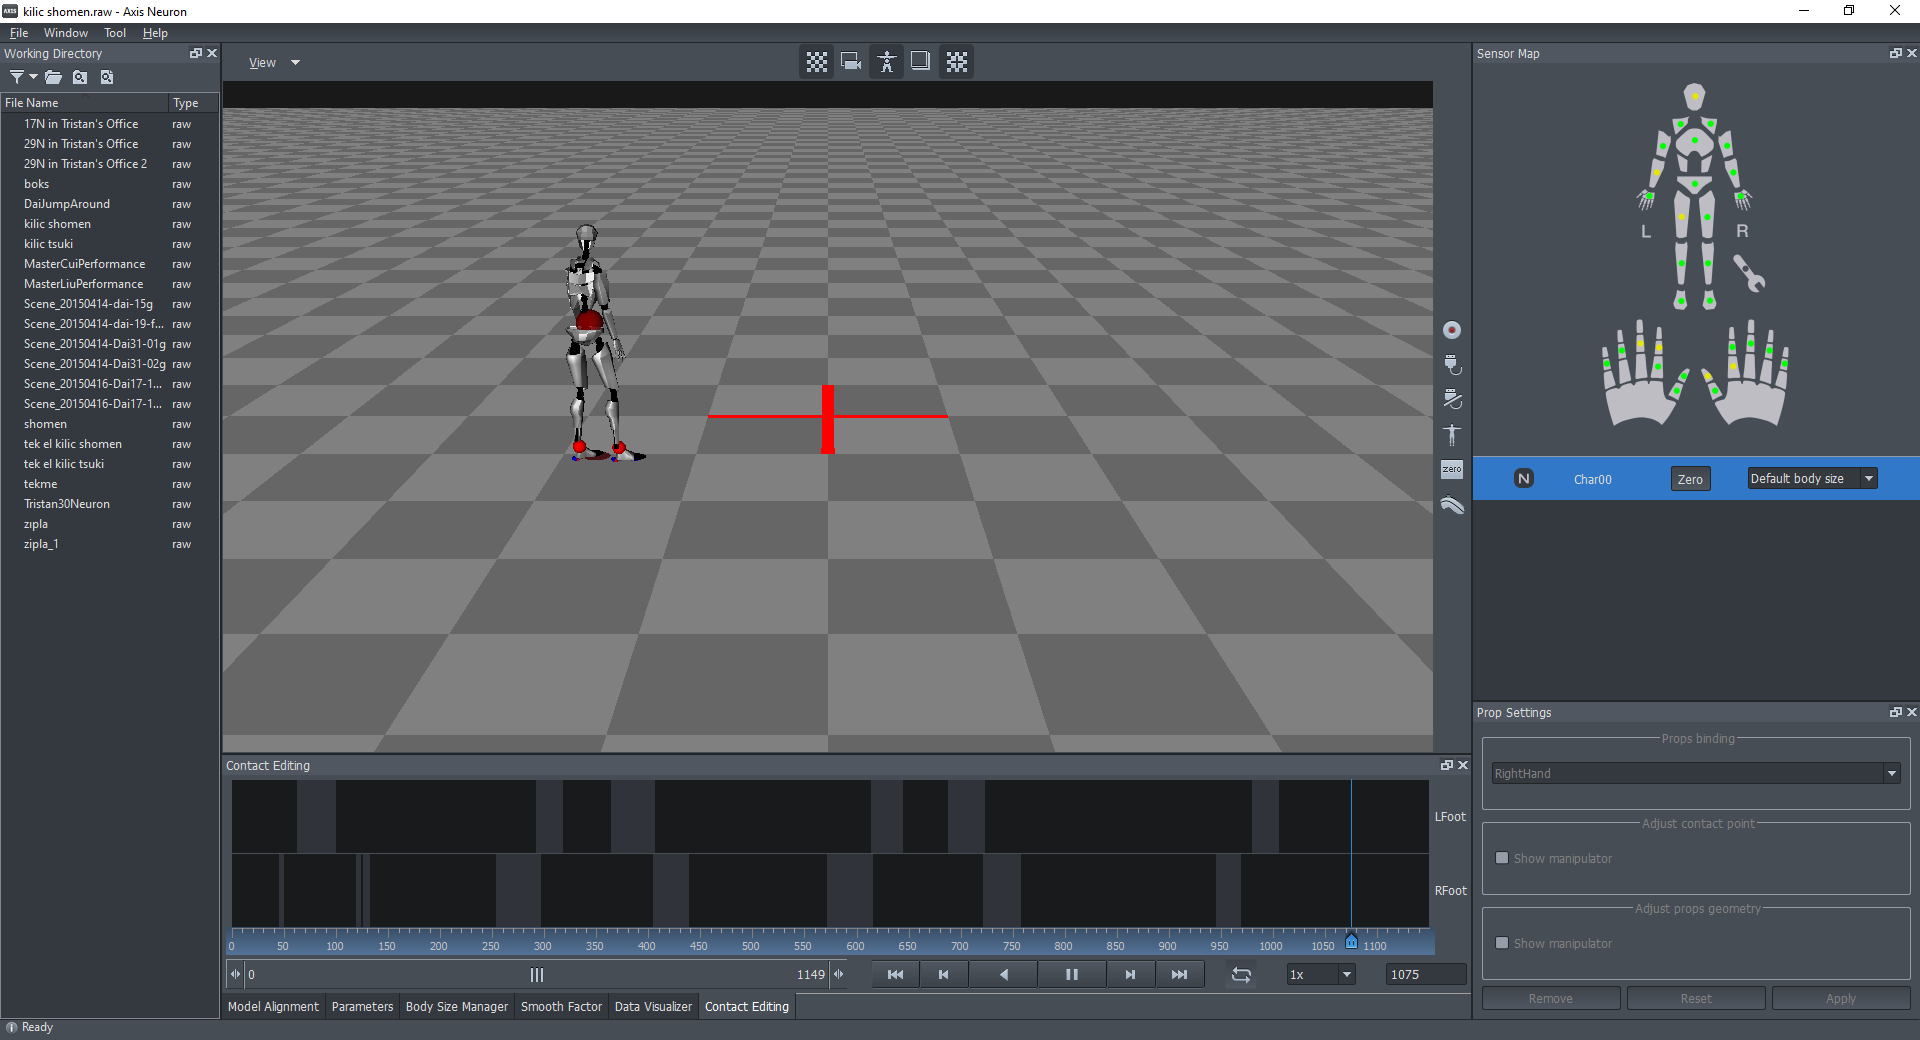
\includegraphics[width=6in]{images/an}
    \caption{Axis Neuron yazılımı}   
    \label{an}
\end{figure}

Perception Neuron, aynı zamanda bir asset paketi halinde bir Unity SDK’sı sunmaktadır. Bu SDK
içerisinde Axis Neuron’da gözüken insansı modelin Unity’de kullanılabilir çeşitli versiyonları ve
bu modelleri Axis Neuron’a bağlayıp hareket verisini takip etmelerini sağlayabilmek için gerekli
kimi betikler mevcuttur. Bu betikler aracılığı ile, Axis Neuron’un ağ üzerinden yaptığı BVH
formatında hareket verisi yayınını Unity SDK’sında bulunan NeuronRobot modellerinden biri veya
uygun iskelet yapısına sahip başka herhangi bir insansı model takip edebilir ve hareketleri Unity
içerisinde aynen taklit edebilir.

\subsubsection{Cardboard}
Google Cardboard; kartondan yapılma, son derece düşük maliyetli, mobil cihazlarla kullanılabilen ve
Google’ın geliştirdiği sanal gerçeklik API’si ve SDK’larından faydalanılarak programlanabilen bir
sanal gerçeklik gözlüğüdür. Gözlüğün yapımı son derece basit olduğu için sayısız üretici tarafından
çeşitli varyasyonları yapılmaktadır, hatta evde bile yapılması mümkündür. Bu projenin
geliştirilmesinde de Şekil \ref{cbjpeg}’te gördüğünüz son derece basit gözlük kullanılmıştır.

\begin{figure}[ht!]
    \centering
        \includegraphics[width=4in]{images/cbjpeg}
    \caption{Projede kullanılan Cardboard sanal gerçeklik gözlüğü}   
    \label{cbjpeg}
\end{figure}

Cardboard içine bir mobil cihaz yerleştirilerek kullanılmaktadır. Bu proje geliştirilirken, Sony
Xperia Z5 Compact Android akıllı telefon bu amaçla kullanılmıştır. Günümüzde tüm akıllı
telefonlarda bulunan ivmeölçer ve jiroskop aracılığı ile uygulama kullanıcının kafa hareketlerini
algılamakta ve bakış açısını ona göre ayarlamaktadır.

\subsubsection{Unity}
\tolerance=659
Unity, Unity Technologies tarafından geliştirilen ve çok sayıda platforma destek veren bir oyun
motorudur. 2 boyutlu ve 3 boyutlu oyun, animasyon veya simülasyon geliştirmek için çok sayıda
içerik üretici tarafından aktif biçimde kullanılmaktadır. Sürükle-bırak formatında araçlarla
uygulama geliştirmeye olanak sağlayan editör arayüzünün yanı sıra, C\# programlama dilinde
Unity’nin geliştiricilere sunduğu API’ler yardımıyla kod yazarak uygulama geliştirmek de mümkündür \cite{unityg}.
Şekil \ref{u}'te Unity’de projenin geliştirilme sürecinden bir ekran alıntısı
görülmektedir.

\begin{figure}[ht!]
    \centering
        \includegraphics[width=5.8in]{images/u2}
    \caption{Unity'de projenin geliştirilme sürecinden bir görüntü}   
    \label{u}
\end{figure}

Google’ın Cardboard cihazlar için sağladığı SDK ve Unity’nin kendi XR API’si projede sanal
gerçeklik ortamının oluşturulması için kullanılmıştır. Projenin Android cihazlara yüklenip
çalıştırılabilecek APK formatında derlenmesi için Android Studio ile birlikte gelen Android SDK’sı
ve Java Development Kit (JDK) kullanılmıştır. Perception Neuron ile entegrasyon ise, Perception
Neuron için geliştirilmiş ve Unity’ye Asset olarak eklenebilen Unity SDK’sı aracılığı ile
gerçekleştirilmiştir.

\subsubsection{Sistem Mimarisi}
Projede kullanılan tüm donanım ve yazılımın entegrasyonu için izlenen süreç, Şekil \ref{ent}’te
verilen akış diyagramında gösterilmiştir.

\begin{figure}[ht!]
    \centering
        \includegraphics[width=6in]{images/ent}
    \caption{Sistem parçalarının entegrasyonu}
    \label{ent}
\end{figure}

Öncelikle, kullanıcının giydiği hareket yakalama cihazından alınan hareket
verisi, kullanıcının bilgisayarına USB veya Wi-Fi üzerinden
aktarılmaktadır. Bilgisayarda çalışmakta olan yazılım, topladığı hareket bilgisini ikili (binary) BVH formatında bilgisayarın
7001 portundan yayınlamaktadır. Burada önemli bir ayrıntı, farklı yönlendiricilere (router) bağlı
uzak bilgisayarlar arasında simülasyonun çalıştırılabilmesi için 7001 portunun dışarıdan erişime
açılmış (yönlendirilmiş) olması gerekliliğidir. 7001 portundan yayınlanan BVH formatındaki hareket
verisi, mobil cihazda çalışmakta olan simülasyon tarafından alınır ve
kullanıcının simülasyon içerisindeki avatarını hareket ettirmek için kullanılır. İki kullanıcı da
birbirlerinin BVH yayınlarından gelen veriyi eş zamanlı olarak takip ederler. Kullanıcılar,
simülasyon içerisinde avatarlarının kafası yerine yerleştirilmiş kameralardan gelen görüntüyü,
sanal gerçeklik gözlüklerini kullanarak görebilir ve kafalarını hareket ettirerek ortamda
çevrelerine bakabilirler.

\subsection{Sistem Gerçeklenmesi}

Proje yazılımının üretiminde, Unity’nin sağladığı sürükle-bırak tarzı araçlar kullanılarak bir
simülasyon ortamı oluşturulmuş, bu ortamda Perception Neuron Unity SDK’sı tarafından sağlanan VR
destekli insan modeli modifiye edilerek kullanılmış ve kullanıcıların bu modelleri kontrolü ve
birbiri ile etkileşimini sağlamak için C\# programlama dilinde betikler yazılmıştır. Bunların yanı
sıra, modifiye edilmiş kimi hazır Assetlerden de faydalanılmıştır.

\subsubsection{Lobi}
\tolerance=750
Uygulama başlatıldığı zaman, kullanıcıları bir lobi ekranı karşılamaktadır. Bu lobi ekranı, Unity
Asset Store’dan ücretsiz edinilebilen ve Unity Technologies tarafından örnek sağlaması amacıyla
geliştirilmiş Network Lobby assetinin bir miktar ekleme yapılmış halidir.

Uygulamada, lobinin DIRECT PLAY başlığı altındaki PLAY AND HOST sekmesi kullanılmaktadır. Bu sekme
kullanılarak kullanıcılardan biri oyun kurucu (host) rolünü üstlenir. Diğer kullanıcı, oyun kurucu
olan kullanıcının, aynı ağ üzerindelerse dahili, farklı ağlara bağlı iseler harici IP adresini JOIN
A GAME kısmındaki kutucuğa yazıp JOIN butonuna tıklayarak lobiye dahil olabilir. Şekil \ref{l1}’da
görülen yeni ekranda ise kullanıcılar, bağlanacakları BVH yayınının IP adresini
kendilerine ait olan kutucuklara yazıp yanındaki JOIN butonuna tıklarlar. İki kullanıcı da JOIN
butonuna tıkladıktan sonra 3 saniye içerisinde simülasyon başlar.

\begin{figure}[ht!]
    \centering
        \includegraphics[width=6in]{images/l1}
    \caption{DIRECT PLAY lobisi, Axis Neuron'un IP adresi girilmiş, yalnızca bir kullanıcı mevcut.}
    \label{l1}
\end{figure}

Lobinin işlevsel kısmını oluşturan LobbyManager objesi üzerinde bir Lobby Manager betiği mevcuttur.
Bu betiğin parametreleri modifiye edilerek simülasyon başladığı zaman kullanıcılar için simülasyon
ortamına çağırılacak model olarak istenen modelin prefab’i verilebilir ve simülasyon ortamı olarak
da istenen sahne sunulabilir. Kullanıcıların girdiği IP adreslerinde yayın yapan Axis Neuron’a
bağlanabilmeleri için bu LobbyManager objesine NetworkLobbyHook isimli bir betik eklenmiştir. Bu
betik içerisinde, lobi sahnesinden simülasyon ortamına geçiş yaparken çağrılacak modeller/prefab’ler
üzerinde, lobi sırasında mevcut bilgiler kullanılarak değişiklik yapılabilmektedir. Betik, lobi
ekranında girilen IP adreslerinin alınıp, kullanıcı avatarını oluşturan objenin/modelin üzerindeki
NeuronAnimatorInstance betiğindeki Address değişkeninin üzerine yazmak için kullanılmaktadır. Bu
sayede kullanıcılar simülasyona girdikleri zaman avatarları, lobideki girdikleri adreslerdeki BVH
yayınından alınan hareketleri izlemektedir.

\subsubsection{Simülasyon Çevresi}

Simülasyon alanı, boş bir düzlemden oluşmaktadır. Bu düzlemde kullanıcılar bir başlangıç noktasında
alana girdikten sonra, kendi avatarlarını vücut hareketlerini takip edecek şekilde yönlendirebilir
ve birbirleri ile etkileşime geçebilirler. İki avatar mevcutken simülasyon alanının dışarıdan
görüntüsü Şekil \ref{env}’de görüldüğü gibidir. Simülasyon alanında harici bir nesne bulunmamasına
karşın, eklenmesi durumunda kullanıcılar çevrelerindeki nesneler ile fiziksel etkileşime (itmek,
çarpmak vs.) geçebilmektedirler. Kullanıcı avatarının gerçeklenmesi için, Perception Neuron Unity
SDK’sı tarafından sağlanan sanal gerçeklik uygulamaları için ayarlanmış NeuronRobot\_MultiMesh isimli
bir insan modeli prefab’i kullanılmıştır. Bu prefab üzerinde yapılan kimi değişiklik ve eklemeler
sayesinde çok kullanıcılı bir sanal gerçeklik ortamında üzerindeki kameranın sıkıntısız çalışması
sağlanmış, çevre nesnelerle fiziksel etkileşime girmesi mümkün kılınmış ve simülasyon mekanikleri
gerçeklenmiş ve avatarın eline simülasyon sırasında kullanabileceği bir kılıç eklenmiştir. Kamera,
fiziksel etkileşim ve oyun mekaniklerinin nasıl çalıştığı ilerleyen kısımlarda daha ayrıntılı
açıklanacaktır.

\begin{figure}[ht!]
    \centering
        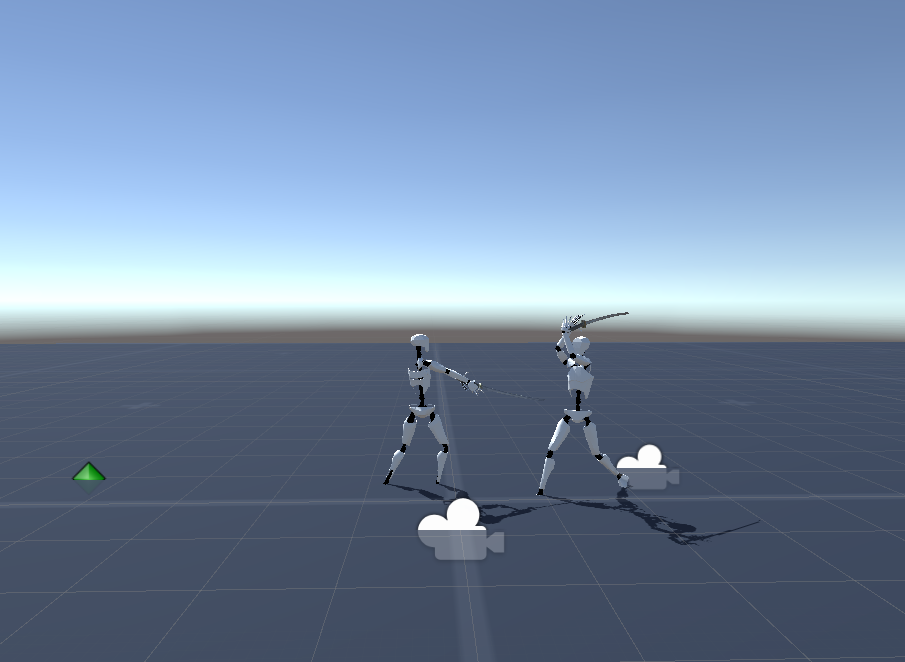
\includegraphics[width=6in]{images/env2}
    \caption{İki avatar ile simülasyon alanı görüntüsü, Unity içerisinde uygulama çalışırken scene
             ekranından alınmıştır.}
    \label{env}
\end{figure}

Avatarın elindeki silah için birden fazla alternatif çözüm denenmiştir. Projenin başında kullanılan
silah, Unity içerisinde tasarlanmış basit bir eliptik silindirdir ve keskin olması gereken kısmında
kapsül şeklinde bir collider Şekil \ref{s}’de en sağda görüldüğü gibi mevcuttur. Şekil \ref{s}’de
görülen diğer silah ise, Unity Asset Store’dan edinilmiş ücretsiz bir assetin modifiye edilmiş
halidir. Bu silahın çelik kısmı, karşıdaki kullanıcının avatarına temas ettiği takdirde karşıdaki
kullanıcının avatarının ölmesine sebep olması beklenmektedir. Bu sebeple çarpışmaları algılaması
için üzerine collider ve fizik kuvvetlerinden etkilenmesi için bir rigidbody eklenmesi gerekmiştir.
Bu aşamada ilk olarak, Şekil \ref{s}’de ortadaki görselde görüldüğü gibi normalde kılıcın kabzası
için tasarlanmış bir convex mesh collider kullanılması tercih edilmiştir. Ancak bu şekilde eklenen
collider, avatarın eline temas edip "kesilmesine" sebep olabildiği için, keskin kısmın saptan bir
miktar daha yukarıda başlaması amacı ile farklı bir collider tasarlanması gerekmiştir. Burada,
amaca uygun bir mesh collider elde etmek için herhangi bir 3D modelleme yazılımı kullanılması
yerine, daha basit bir çözüm olarak iki adet basit dikdörtgen şeklinde collider Şekil \ref{s}’de en
baştaki görselde görüldüğü gibi kullanılmıştır. Bu çözüm, yalnızca keskin kısmın ele çok yakın
olması problemini çözmekle kalmamış, aynı zamanda kılıcın normalde keskin olmaması gereken arka
kısmında collider bulunmamasına imkan sağlamıştır. Şu an projenin son halinde bu silah
kullanılmaktadır.

%Avatarın elindeki silah için birden fazla alternatif çözüm denenmiştir. Projenin güncel haline
%kullanılan silah, Unity içerisinde tasarlanmış basit bir eliptik silindirdir ve keskin olması
%gereken kısmında kapsül şeklinde bir collider Şekil \ref{s}’de görüldüğü gibi mevcuttur. Şekil
%\ref{s}’de görülen diğer silah ise, Unity Asset Store’dan edinilmiş ücretsiz bir assetin modifiye
%edilmiş halidir. Bu silahın çelik kısmı, karşıdaki kullanıcının avatarına temas ettiği takdirde
%karşıdaki kullanıcının avatarının ölmesine sebep olması beklenmektedir. Bu sebeple çarpışmaları
%algılaması için üzerine bir mesh collider ve fizik kuvvetlerinden etkilenmesi için bir rigidbody
%eklenmesi gerekmiştir. Ancak, kılıcı tutan avatarın kendisini öldürmesine engel olmak için mesh
%collider’ın yalnızca kılıcın çelik kısmını kapsaması gerekmektedir. Bu amaçla kılıca, tamamını
%kaplayan bir mesh collider yerine, kabzası için tasarlanmış ve yalnızca çelik kısmın etrafını
%kapsayan bir mesh collider eklenmiştir. Rigidbody’nin düzgün çalışabilmesi için bu mesh collider
%convex olarak ayarlanmıştır. Bu silahın şu anda kullanılmamasının sebebi ise rigidbody ile ilgili
%bir problemden kaynaklı olarak simülasyon başladığında silahın aşağı düşmesidir. Bu silahın
%rigidbody’li ve rigidbody’siz hallerini kullanan avatarlar da farklı prefab’ler olarak proje
%dosyaları içerisinde mevcuttur (NeuronRobot\_MultiMesh\_sword\_rb ve
%NeuronRobot\_MultiMesh\_sword\_norb).

\begin{figure}[ht!]
    \centering
        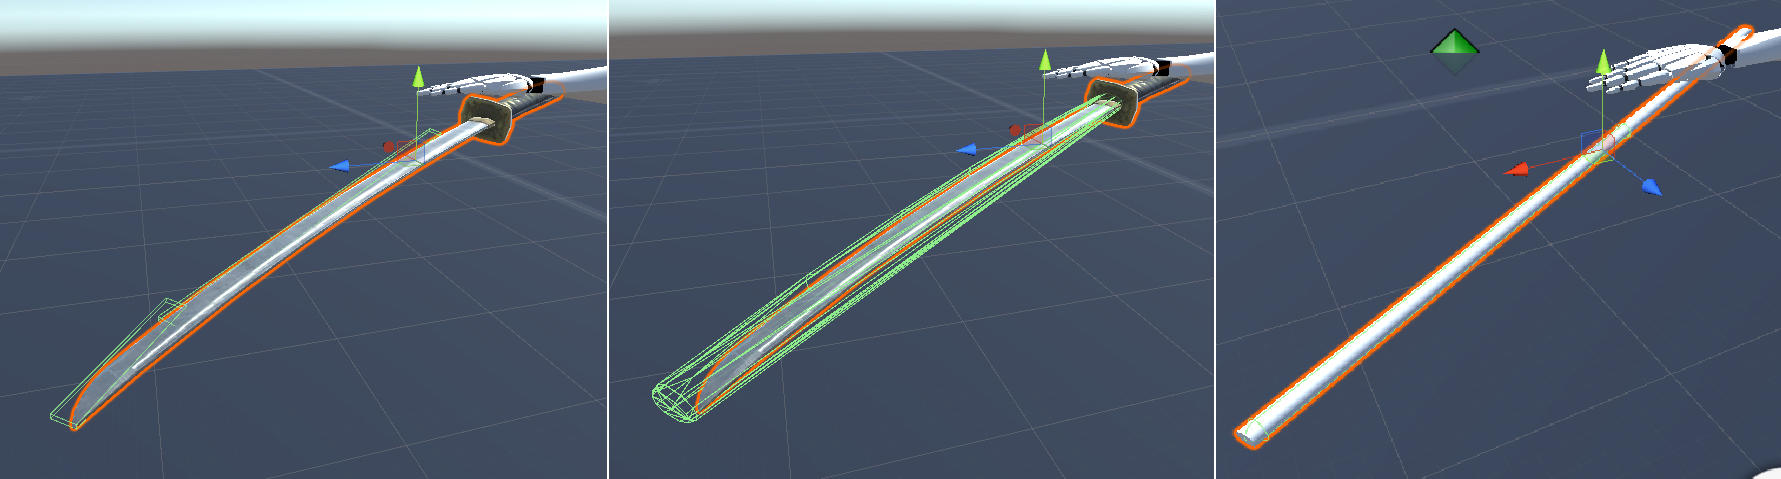
\includegraphics[width=6in]{images/s2}
    \caption{Solda: Asset Store'dan edinilip modifiye edilen kılıç ve iki adet basit box(kutu)
             collider. Ortada: Kabzasının convex mesh collider'ını kullanan kılıç. Sağda: Unity
             içerisinde tasarlanan silah.}
    \label{s}
\end{figure}

Bu şekilde avatarın eline sabitlenmiş bir silah kullanılmasının sebebi, Perception Neuron’un el ve
parmak hareketlerini algılamadaki hassasiyetinin ve Unity fizik motorunun çok küçük kuvvet
değişimlerini hesaplama kabiliyetinin söz konusu silahı kullanıcının hareket yakalama aracılığı ile
elinde tutabilmesi için yetersiz olmasıdır. Projenin ilerleyen iterasyonlarında, kullanıcının
kılıcı iki eli ile daha yüksek hareket özgürlüğü ile tutabilmesi için farklı mekanizmalar
geliştirilecektir.

\subsubsection{Çarpışmalar ve Fizik Motoru}
Perception Neuron Unity SDK’sı, insan modellerine rigidbody eklemek için Skeleton Tools isimli bir
araç sunmaktadır. Ancak SDK’nın güncel sürümlerinde aynı aracı collider eklemek için kullanmak
mümkün değildir. Proje boyunca bu konuda doküman eksikliği sebebiyle sıkıntılar yaşanmıştır.
Sonunda sorun, insan modeli objesinin uygun çocuk objelerine convex collider’ların Şekil \ref{c}’da
görüldüğü gibi tek tek eklenmesi ile çözülmüş ve kullanıcı avatarının çevresindeki nesneleri
manipule edebilmesi mümkün kılınmıştır. Bunun bir sonraki aşaması ise, çarpışmaların simülasyon
içerisindeki kılıç temasında ölme gibi mekaniklerin işlenebilmesi için kullanılması olmuştur. Bu
aşamada yaşanan önemli bir sorun, Unity’nin çarpışma algılama mekanizması sebebiyle collider’lar
tarafından algılanan çarpışmaların obje hiyerarşisinde içinde rigidbody barındıran en yakın
üst (parent) nesne tarafından işlenmesi sebebiyle ortaya çıkmıştır. Bu çarpışmaların algılanıp
işlenebilmesi için, içinde rigidbody bulunan yani çarpışma verisininin iletildiği tüm nesnelerin
içerisine çarpışmaları algılayacak Stabbed isimli bir betik eklenmiştir. Kullanıcıların tüm
eklemleri, “Player” etiketine sahip nesnelerdir; ellerindeki kılıçlar ise “weapon” etiketine
sahiptir. Çarpışma algılama betiği, kendi etiketi Player ise ve çarptığı nesnenin etiketi weapon
ise, kendisinin bağlı olduğu kök nesneye bağlı Player betiğindeki Die() metodunu çağırarak bağlı
olduğu oyuncu avatarının ölmesini sağlar. Player betiğinin içerisindeki Alive isimli bir boolean
değer avatarın canlı olup olmadığını takip ederek, birden fazla eklemle çarpışma halinde Die()
metodunun birden çok kez çağrılmasına engel olur. Şekil \ref{col}’daki şema da bu mekanizmayı
açıklamaktadır.

\begin{figure}[ht!]
    \centering
        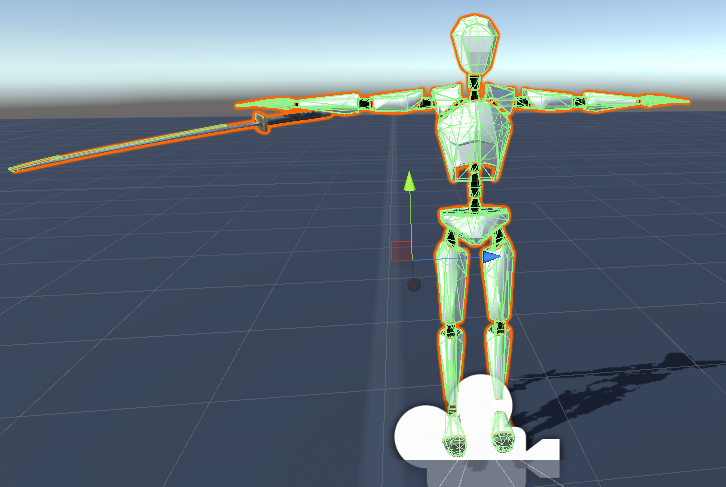
\includegraphics[width=5in]{images/c2}
    \caption{Avatarın tüm beden parçalarına eklenen collider'lar}
    \label{c}
\end{figure}

\begin{figure}[ht!]
    \centering
        \includegraphics[width=6in]{images/col}
    \caption{Çarpışmaların çalışma mekanizması.}
    \label{col}
\end{figure}

\subsubsection{Ağ Üzerinden Kullanıcıların Bağlanması}
\tolerance=1708
Uygulamada kullanıcılar arası ağ bağlantısı kurma amaçlı Unity’nin sağladığı Multiplayer High
Level API ve diğer ağ özelliklerinden faydalanılmıştır. Projenin başlarında, oyuncular arası
bağlantının tamamiyle bu yapı üzerinden, bir sunucu-istemci yapısı kullanılarak gerçeklenmesi
planlanmıştır. Ancak ilerleyen kısımlarda bu yapıdan vaz geçilip, bunun yerine yalnızca hareket
verilerinin aktarıldığı, bunun da Unity’nin sunduğu ağ özelliklerinden faydalanmak yerine BVH
formatında yayınlanan hareket verilerine iki kullanıcının da direkt olarak kendi yerel
makinaları üzerinden bağlandığı bir sistem kullanılmıştır. Uygulama içerisinde Unity’nin ağ
özelliklerinden yalnızca Lobi sahnesinde ve simülasyon içerisinde kullanıcıların doğma ve yeniden
doğma süreçlerinde faydalanılmıştır. Bunun haricinde uygulamanın geri kalan kısımları, asenkron
biçimde kullanıcıların kendi lokal makinalarında çalışmaktadır. Bu çalışma prensibi Şekil
\ref{net}’de basitçe gösterilmiştir.

\begin{figure}[ht!]
    \centering
        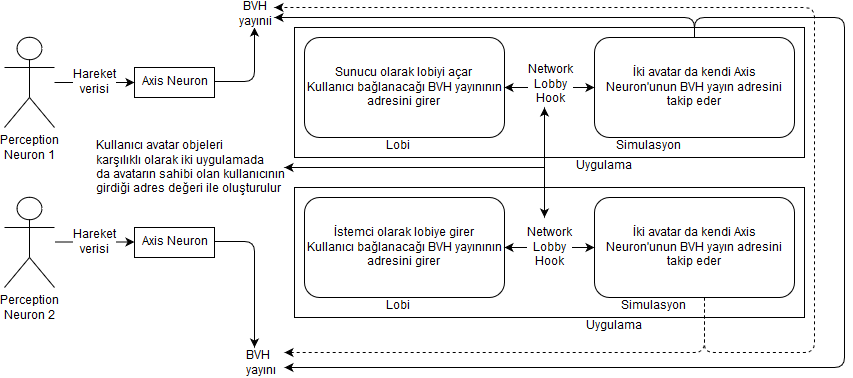
\includegraphics[width=6in]{images/net}
    \caption{Kullanıcı hareketlerinin aktarılması. Görüldüğü üzere iki uygulama da iki kullanıcının
             avatarlarına ait BVH verisini direkt olarak o kullanıcıya ait Axis Neuron yazılımından
             almaktadırlar.}
    \label{net}
\end{figure}

Tam senkronize bir çoklu kullanıcı yapısı yerine bu şekilde sadece hareket verisinin aktarıldığı ve
tüm hesaplamaların lokal makinalarda yapıldığı bir yapı tercih edilmesinin altında üç temel
motivasyon yatmaktadır: Birincisi, tüm eklemlerinin hareket verisini bir hareket yakalama cihazının
yayınladığı verilerden alan ve gerçekçi fizik özelliklerine sahip olması gereken bir avatarın tüm
eklemlerinin hareketlerini ağ üzerinden aktarmak mümkün ancak karmaşık bir işlemdir. İkincisi, bu
şekilde hareket verisinin Axis Neuron’dan yazılan uygulamaya, oradan da işlenip uygun biçimde ağ
üzerinden uzaktaki makineye aktarılması ve sunucu-istemci arasındaki istek-yanıt süreçleri
uygulamaya çok ciddi gecikme süreleri ekleyip, bir simülasyonda olması gereken gerçekçiliği elde
etmeyi zorlaştıracaktır. Üçüncüsü de, her ne kadar kullanıcıların uygulamayı asenkron biçimde kendi
makinalarında çalıştırıyor olmaları lokal modifikasyonlara ve hile yapmaya çok ciddi olanak sunsa
da, unutulmamalıdır ki gerçeklenmeye çalışılan uygulama rekabetçi bir oyun değil, eğitim ve çalışma
amaçlı bir simülasyondur. Rekabetçi bir puan sistemi bulunmamaktadır ve amaç, rakibi yenmek değil,
karşılıklı çalışmaktır. Dolayısıyla kullanıcıların hile yapmasına imkan sağlanması aslında önemli
bir problem değildir, gecikmeleri düşürüp gerçekçiliği korumak çok daha önemli bir kıstastır.

Perception Neuron’dan alınan verilerin ağ üzerinden aktarılması, iki kullanıcının, uygulamanın iki
cihazdaki asenkron çalışan örneklerinin ikisinde de avatarlarına bağlı olan NeuronAnimatorInstance
betiklerindeki address değişkeninin kendi Axis Neuron’larının yayın yaptığı adresi tutması ile
mümkün kılınmıştır. Bu da yukarıda Lobi bölümünde de anlatıldığı gibi, Lobi ekranında girilen
adresin çekilip simülasyon ekranına geçiş aşamasında oluşan kullanıcıya ait avatara aktarılması ile
sağlanmıştır. Söz konusu betik Perception Neuron Unity SDK’sı tarafından sağlanmış olmasına karşın,
bu şekilde çalışabilmesi (iki kullanıcı için ayrı address değerleri tutabilmesi) için bu script
içerisinde tanımlanan NeuronAnimatorInstance sınıfının temel aldığı (kalıtıldığı/inherit edildiği)
NeuronInstance sınıfının bulunduğu betikte kimi değişiklikler yapılması gerekmiştir. Sınıf,
MonoBehaviour yerine NetworkBehaviour sınıfını temel alacak şekilde düzeltilip, address değişkeni
ve kimi başka değişkenler SyncVar olarak yeniden tanımlanmıştır.

Bunun haricinde ağ kullanan özellikler, kullanıcı avatarlarına ait mekaniklerin tanımlandığı Player
isimli betik içerisindeki başlama ve ölünce yeniden doğmayı kontrol eden Start() ve Respawn()
metotları ile kameraların aktive edildiği EnablePlayer() metodlarıdır. Bu metotlarda kullanıcının
sunucu veya istemci olmasına bağlı olarak (her ne kadar tam olarak bir sunucu-istemci sistemi
kullanılmasa da Unity için kullanıcılardan biri sunucu diğeri istemcidir) simülasyon alanında
doğacakları nokta belirlenir ve iki avatardan sadece o anda kontrol edilenin kamerası
aktifleştirilir.

\subsubsection{Simülasyon Akışı ve Mekanikler}

Bu kısımda simülasyon sahnesine geçildikten sonra uygulamanın çalışma akışı ve mekanikleri
açıklanmıştır.

Simülasyonun kullanıcılar için akışını, iki kullanıcının da avatarına eklenmiş olan Player isimli
betik belirlemektedir. Betiğin nasıl çalıştığı Şekil \ref{player}'deki akış diyagramında da
gösterilmiştir.

Bu betik içerisindeki Start() metodu başlangıcı belirler. Öncelikle iki kullanıcı da önceden
belirlenmiş sabit bir konumda doğacak şekilde ayarlanırlar: Sunucu için (0, 0, 0) ve istemci için
(0, 0, 2). Ardından betiğin bağlı olduğu kullanıcı avatarını çalıştıracak EnablePlayer() metodu
çağırılır.

EnablePlayer() metodu içerisinde, avatarı aktifleştirmek için öncelikle kullanıcının görüşünü
sağlayacak, avatarın kafası yerine yerleştirilmiş kamera aktive edilir. Ardından avatara bağlı olan
NeuronAnimatorInstance betiği aktive edilir ve Axis Neuron ile bağlantısı kurulur.

Simülasyon bu şekilde başlar ve kullanıcılar avatarlarını kontrol ederek ellerindeki kılıçlar
yardımıyla birbirlerine karşı hamle yapabilirler. Kılıçların oyunculara temas edip etmediği ise,
üzerinde rigidbody bulunan tüm vücut parçalarına eklenmiş olan Stabbed betiği ile kontrol edilir.
Simülasyon içerisinde yalnızca kılıçlar “weapon” olarak etiketlenmiştir, oyuncu avatarlarının tüm
parçaları ise “Player” olarak etiketlenmiştir. Stabbed scripti, bağlı olduğu nesne “Player”
etiketine ve çarptığı nesne “weapon” etiketine sahipse çalışır, ve kendisinin bağlı olduğu nesnenin
en üst atası (root) olan kullanıcıya bağlı Player betiği içerisinde yer alan Die() metodunu
çağırarak çarpışmanın gerçekleştiği avatarın ölmesini sağlar. Birden fazla eklemin çok kısa
aralıklarla çarpması durumunda Die metodunun birden çok kez çağrılmasını önlemek için avatarın
hayatta olup olmadığını takip eden bir boolean değişken tutulmaktadır. Kılıcın sapı ile temasın
silahın sahibi olan avatarı öldürmesine engel olmak için de kılıcın mesh collider’ı olarak kılıcın
tamamını kapsayan kendi collider’ı yerine yalnızca çelik kısmın etrafını kapsayan kabza için
tasarlanmış collider kullanılmıştır.

Avatarı öldüren Die() metodu ise, avatarı kullanılmaz hale getirmek için DisablePlayer() metodunu
çağırdıktan sonra, 3 saniye içerisinde yeniden doğması için Respawn() metodunu gecikmeli olarak
çağırır.

DisablePlayer() metodunun ise tüm yaptığı, kullanıcını kamerasını ve NeuronAnimatorInstance
betiğini deaktive ederek ekranının kararmasını sağlamak ve avatarını kontrol etmesine engel
olmaktır.

Bunun ardından çağrılan Respawn() metodu, kullanıcının simülasyona başlama pozisyonunu tekrar
ayarlar ve ReEnablePlayer() metodunu çağırır.

Son olarak da ReEnablePlayer() metodu, simülasyonun başlangıcı için yapılması gereken bazı ekstra
adımları atlamak şartıyla EnablePlayer() metodunun yaptıklarının birebir aynısını yapar: kullanıcı
kamerası ve NeuronAnimatorInstance betiğini yeniden aktifleştirir.
\newpage
\vfill

\begin{figure}[ht!]
    \centering
        \includegraphics[width=6in]{images/player}
    \caption{Player betiği için akış diyagramı.}
    \label{player}
\end{figure}

\vfill
\clearpage

\subsubsection{Sanal Gerçeklik}

Sanal gerçeklik kısmının gerçeklenmesi için Google Cardboard SDK’sından, Unity’nin XR API’sinden ve
Perception Neuron Unity SDK’sının içinde bulunan sanal gerçeklik örneklerinden faydalanılmıştır.
Uygulama ilk açıldığı sırada kullanıcının karşısına çıkan lobi ekranı sanal gerçeklik
kullanmamaktadır. Bunun bir numaralı sebebi, sanal gerçeklik kullanırken IP adresi girmenin
kullanıcı açısından yaratacağı zorluktur. Simülasyon başladığında ise, sanal gerçeklik moduna
otomatik olarak geçilmektedir.

Perception Neuron Unity SDK'sı tarafından sağlanan sanal gerçeklik örneğinde kullanılan insan
modelinin kafası yerine kamera koyulmuştur. Ancak uygulamada kamera hala aynı konumda mevcutken
modelin kafası tekrar yerine eklendiğinde kullanıcının görüşünde bir sıkıntı olmadığı fark
edilmiştir. Bu sebeple, kafasıyla beraber bütün bir insan modeli kullanılmıştır. Modelin kafasının
olduğu konuma aynı zamanda bir kamera mevcuttur. Bu kamera, Camera Holder isimli bir GameObject’in
çocuk objesi olarak ayarlanmıştır. Camera Holder ise, yukarıda bahsedilen sanal gerçeklik
örneklerinde kullanılan Neuron VR Adapter isimli bir betiğe sahiptir. Bu betik, kameranın bakış
açısı olarak telefonun yönelişini baz almasını, konum olarak ise avatarın kafasının bağlı olduğu
bağlantı noktasını takip etmesini sağlar. Örnekten farklı olarak, bu projede Camera Holder bağımsız
bir nesne olarak değil, avatarın bir çocuk objesi olarak gerçeklenmiştir. Bunun sebebi, avatarın
önceden simülasyon alanında bulunan değil, doğan (spawn olan) bir nesne olmasıdır.

Lobiden sonra sanal gerçekliğe geçme mekanizması için ise Camera Holder’ın çocuk objesi olan
kameraya VR Toggle isimli bir betik eklenmiştir. Bu betik basitçe, kamera yaratıldığı zaman
(Start() metodunda)) Unity XR’ın kullandığı sanal gerçeklik SDK’sını "None”dan (“hiçbiri”nden)
"cardboard”a çevirmektedir. Kamera yokedildiğinde ise (OnDestroy() metodunda) sanal gerçeklik
modundan SDK'yı tekrar "None"a çevirerek çıkılmasını sağlar. Sanal gerçeklik moduna geçildiğinde
oyun içi bir görüntü Şekil \ref{vr}’te görülebilir.

\begin{figure}[ht!]
    \centering
        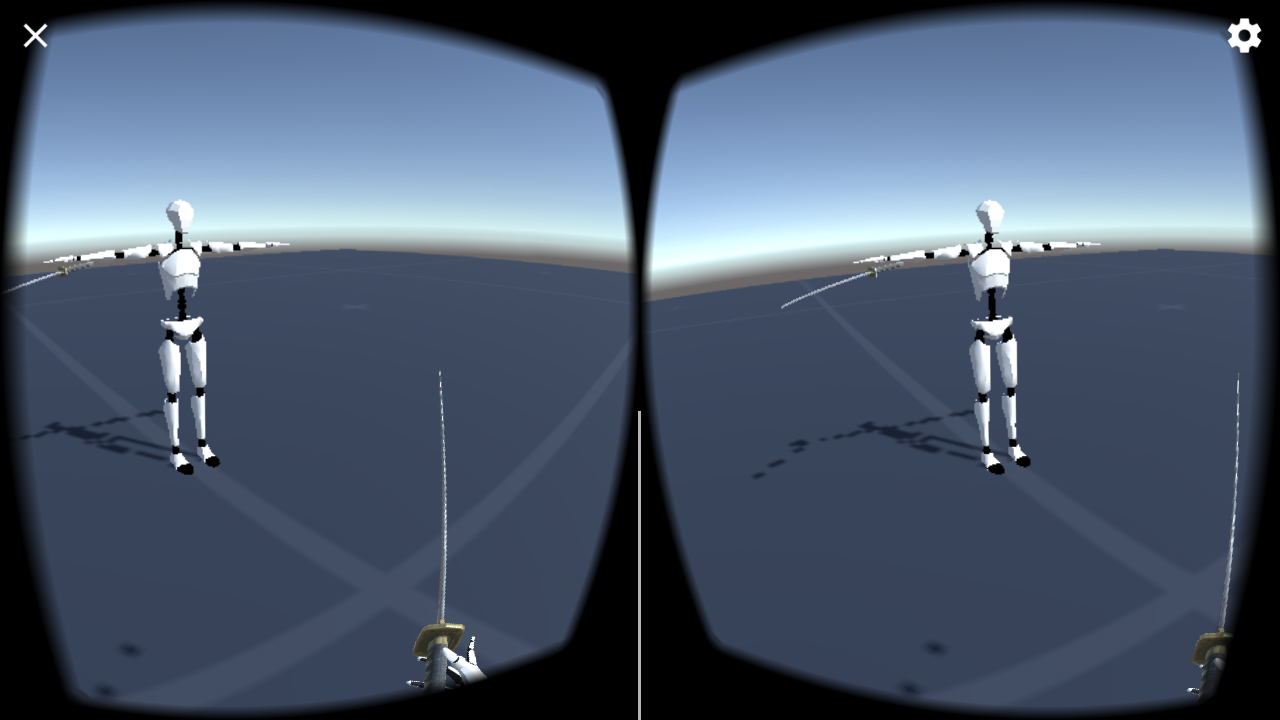
\includegraphics[width=5in]{images/vr2}
    \caption{Sanal gerçeklikle oyun içi bir görüntü. Karşıda görünen avatar herhangi bir Axis        
             Neuron'a bağlanmamış.}
    \label{vr}
\end{figure}

\newpage
\section{Test Ortamı ve Testler}
Gerçekleştirilen testlerde geliştirilen sistem üç aikido sporcusuna denetilmiştir. Deneklerden
ikisi ileri seviye öğrenci, diğeri ise asistan eğitmendir. Bu aşamaya kadar sistem daha önce iki
mobil cihaz arasında hareket yakalama sistemleri ile birlikte denenmediği için, bu deney süreci hem
deney hem de hata ayıklama süreci olarak işlev görmüştür. Sistemdeki çok sayıda daha önceki
testlerde fark edilmemiş hata bu süreçte düzeltilmiştir.

\subsection{Test Ortamı}
Testler, üç denek ile kapalı bir mekanda gerçekleştirilmiştir. Öncesinde bir oda içerisinde, ardından
daha geniş bir koridorda test edilmiştir sistem. Denekler ikili gruplar halinde sistemi denemişlerdir.
İki adet Perception Neuron hareket yakalama cihazı ve biri Cardboard diğeri ise Freefly VR olmak üzere
iki adet sanal gerçeklik gözlüğü kullanılmıştır. Deneyler, iki telefon aynı Wi-Fi ağına bağlı iken
gerçekleştirilmişlerdir. Bir mobil cihazın taşınabilir Wi-Fi hotspot özelliği kullanılmış ve testler
3G ve LTE bantları üzerinde gerçekleştirilmiştir. Uygulama, Sony Xperia Z5 Compact ve Samsung Galaxy
S4 akıllı telefonlarında Android 5.1 ve 7.1 işletim sistemleri üzerinde denenmiştir.

Test ve hata ayıklama süreçleri birlikte yürütülmüştür. Deneklerin dahil olduğu iki günlük süre boyunca
sürekli olarak sistem test edilmiş, bulunan hatalar düzeltilmiş ve tekrar test edilmiştir.

\subsection{Testler}
Testler sırasında öğrencilerden biri, sırasıyla diğer öğrenci ve eğitmenle karşılıklı olarak simülasyona
girmiştir. İki kişi karşılıklı mücadele etmeye çalışmıştır.

Testler sırasında sistemde hala düzeltilmesi gereken hatalar olmakla birlikte, genel olarak başarılı
olduğu ortaya konmuştur. Denekler sistemi iki gün boyunca test etmiş ve sonunda on soruluk bir ankete
cevap vermişlerdir. Sonuçlar sistemin hala geliştirilmesi gerektiğini ancak ileride savaş sanatları
eğitiminin bir parçası olmak için umut vadettiğini ortaya koymuştur.

Testler iki cihaz aynı ağa bağlıyken sistemdeki gecikme miktarının ihmal edilebilir düzeyde olduğunu
da göstermiştir.

Testler sırasında ortaya çıkan ve düzeltilmesi gereken önemli sorunlardan biri, hareket yakalama
cihazından gelen vücut doğrultusu bilgisi ile akıllı telefonun jiroskopundan gelen kafa doğrultusu
verisi arasındaki uyumsuzluktur. Her bir kaç denemede bir, kullanıcılardan birinin simülasyonda gördüğü
alan ile vücudunun baktığı doğrultunun uyumsuz olduğu gözlemlenmiştir.

Kullanılabilirlik konusunda ise, kılıcın ele sabitlenmiş olması,
özellikle eldeki sensörlerin kalibrasyonunda bir kayma olduğu zaman kılıcın kontrolünü
zorlaştırmaktadır. Bununla ilgili çözüm önerileri ileride tartışılacaktır.

Testlerin sonunda deneklerin ikisine on soruluk bir anket yapılmıştır. Ankette sistem ile iligli kimi
tespitlerde bulunulmuştur ve katılımcılardan 1 "Kesinlikle Katılmıyorum" ve 5 "Kesinlikle Katılıyorum"
anlamına gelmek üzere tespitlere 1-5 arasında puan vermeleri istenmiştir. Tespit, sistem
kullanabilirliği ölçütü (SUS) anketlerine benzer şekilde bir olumlu bir olumsuz olarak hazırlanmıştır.
Sonunda verilen cevaplar üzerinden standart sistem kullanabilirliği ölçütü kullanılarak bir puan
hesaplanmıştır. Ankette sunulan tespitler şu şekildedir:

\begin{itemize}
    \item Simülasyon yeterince gerçekçiydi
    \item Karakterimi kontrol etmek zordu
    \item Tepki süreleri kısa ve gecikme azdı
    \item Uygulamayı kullanmaya başlamak çok zahmetliydi
    \item Uygulamayı kullanırken çok keyif aldım
    \item Uygulamayı kullanabilmek için ciddi miktarda teknik bilgiye ihtiyaç duydum
    \item Bu sistemin savaş sanatları eğitiminde (öğrenci veya eğitmen olarak) kullanılmasının faydalı olacağını düşünüyorum
    \item Bu sistemin işe yarar bir alternatif antrenman yöntemi olarak kullanılamayacağını düşünüyorum
    \item İmkanım olsa bu sistemi sıkça kullanırdım
    \item Uygulamanın çalışmasında ciddi tutarsızlıklar vardı
\end{itemize}

Her tespitin anket sonucuna göre puan katkısı hesaplanmıştır. Olumsuz tespitler için puan katkısı
"5 - ortalama puan" şeklinde, olumlular için ise "ortalama puan - 1" şeklinde hesaplanmıştır. Sonuç
olarak elde edilen puan katkıları toplanıp 2,5 ile çarpıldığında ise sonuç puanına ulaşılmıştır: 77,5.
Bu puan, sistem kullanılabilirliği ölçütüne göre "iyi" sınıfına girmektedir.


\newpage
\section{Kıyaslamalı Değerlendirme ve Tartışma}
Önceki çalışmalara kıyasla, bir ağ yapısının kullanılması, sitemin karmaşıklığını arttırmış ve
hataların çözülmesini daha zor hale getirmiştir. Buna rağmen, bir konseptin ispatı olarak başarılı
bir sistem elde edilmiştir.

Bu projenin ilham kaynaklarından biri olan, Hareket Yakalama ile
Sanal Gerçeklikte Tenis Oyunu [5] projesi ile nitel bir kıyaslama yapmak mümkündür. Sözü edilen
projede, tek kişilik bir oyun alanında sanal gerçeklik kullanılarak tek kişilik bir tenis oyunu
simülasyonu gerçeklenmiştir. Bu yeni projenin bunun üzerine koyduğu en önemli unsur, ağ üzerinden
bağlı birden fazla kullanıcının varlığıdır. Bu, daha ilerleyen çalışmalarda, rekabetçi oyunlardan
birlikte yapılması gerekecek fiziksel aktivitelere çok sayıda uygulamaya alan açmaktadır.

\newpage
\section{Sonuç ve Gelecek Çalışmalar}
\tolerance=6000
Bu projede iki kişinin ayrı konumlardan bağlanıp karşılıklı olarak çalışabileceği bir savaş
sanatları simülasyonu yapılması amaçlanmıştır. Şimdilik, projenin kapsamı genel bir savaş sanatları
simülasyonundan ziyade, kılıç dövüşü ile kısıtlı tutulmuştur. Amaç, iki kişinin karşılıklı olarak
gerçekçi bir simülasyon ortamının içerisinde normal koşullarda gerçek silahlarla çalışamayacakları
biçimde kılıçla mücadele tekniklerini çalışabilmeleridir. Sonuç olarak elde edilen üründe bu amaç
gerçeklenmiştir. Elbette düzeltilebilecek, ek yapılabilecek, eniyilenebilecek çok sayıda noktası
olmakla beraber; bütün bunların üzerine inşa edilebileceği sağlam bir temel oluşturulmuştur.

Bu noktada artık, elde edilen uygulamanın hangi eksiklerinin kapatılabileceği ve üzerine nasıl
gelişmeler yapılabileceğini tartışmak gerekir.

İlk olarak, daha uzun ve kapsamlı bir test ve hata ayıklama süreci sonunda sistemdeki mevcut
eksiklerin giderilmesi gerekmektedir. Sık yaşanan bakış-duruş uyumsuzluğu sistemin bir numaralı
problemidir ve çözülmeyi beklenmektedir. Bunun haricinde, daha nadir yaşanan ağdan düşme veya
uygulama örneklerinin birisinin hareket yakalama cihazına bağlanamaması gibi sorunlar mevcuttur.
Tüm bu sorunların çözümü ancak daha çok deney, kayıt dosyalarının tutulması ve özenli hata ayıklama
ile mümkündür.

Kullanıcı deneyimini arttırmak için ise bu projeye yapılabilecek kimi eklemelerden burada bahsetmek
gerekiyor. Öncelikle, kullanılabilirliği ciddi anlamda düşüren silahın ele sabitlenmesi problemi
için bir çözüm önerisi: kılıcın sapını iki ele bağlı eksenler etrafında döner hale getirmek.
Aikidoda, kılıç kullanımının esaslarından birisi kılıcı sabit bir biçimde tutmak yerine, bir
kaldıraç misali bir eli destek noktası diğer eli ise kuvvet kolu yaparak hamle yapmaktır. Bu
prensip bu projeye uygulanabilir, kılıcın sağ elde bir eksen etrafında dönmesi sol elin ise bu
dönüşü kontrol etmesi şeklinde bunu gerçeklemek mümkün.

İkinci bir kullanıcı deneyimi arttırıcı iyileştirme de muhakkak silah dizaynı ile ilgili olacaktır.
Şu an mevcut silahlar birbiriyle çarpışamamakta, birbirinin içinden geçmektedir. Aynı zamanda, her
ne kadar colliderlar sadece silahın keskin kısmında olsa da, silah bedenin içinden geçebildiği için
keskin olmayan tarafla vurararak da rakibi öldürmek mümkündür. Bu sorunların çözülmesi için
silah ve silahla ilgili fizik özellikleri ile ilgili çalışma yürütülmelidir.

Bunların haricinde yapılabilecek önemli bir ekleme ise, kapsamı kılıç dövüşünün dışına çıkarıp,
yumruk tekme gibi saldırıların ve bunlara karşı blok alma mekanizmalarının gerçeklenmesi olacaktır.
Burada temas halinde direkt ölmekten ziyade, bir puan veya kalan can sistemi kullanılabilir.

Son olarak akla gelen olası geliştirmeler, daha iyi (mümkünse sanal gerçeklikle uyumlu çalışan) bir
lobi ekranı ve kimi kozmetik iyileştirmeler olacaktır.

Burada sayılan yapılabilecek düzeltme ve geliştirmelerin hepsi bu projenin devamı için yakın
zamanda uygulanması planlanan iyileştirmelerdir.

Bu projenin iyileştirilmesinin yanı sıra, burada gösterilen teknolojiler ve sistem mimarisi taban
alınarak yeni projeler de geliştirilebilir. Farklı spor dalları veya fiziksel aktiviteler için benzer
sistemler kurmak mümkündür. Neredeyse bütün çok oyunculu spor oyunları, hareket yakalama ve sanal
gerçeklik sayesinde gerçek bir sportif aktiviteye dönüştürülebilir.

Bu raporda bahsedilen sistemde de, farklı bedensel aktiviteler için ileride kurulabilecek çok kullanıcılı
hareket algılama sistemlerinde de karşılaşılacak en önemli sorunlardan birisi kurllanıcıların çarpışması
sorunudur. Bu tarz sistemlerde kullanıcıların birbirine çarpması gibi etkileşimler gerçekçi fizik kuralları
ile gerçekleştirilemez, çünkü bu durum simülasyon içerisindeki fizik işlemlerinin sonucu ile hareket
yakalama cihazından gelen hareket verileri arasında bir çelişkiye sebep olacaktır. Kullanıcı simülasyon
ortamında aynen yerinde fizikten etkilenip ona göre konum alırken, gerçek hayatta etkilenmeyecektir. Bu
soruna karşı sunulabilecek bir çözüm önerisi şu olabilir: simülasyonda kullanıcılar arası bir çarpışma
algılandığı zaman çarpışan kullanıcının hareket yakalama cihazı ile bağı bir süreliğine kesilip o sırada
önceden belirlenmiş bir çarpışma animasyonu oynatılabilir. Animasyon oynatıldıktan sonra, kullanıcı
avatarının kontrolü tekrardan hareket yakalama cihazına aktarıılır. Bu yöntemin, yukarıda da bahsedilen
yumruk tekme gibi vuruşların da olduğu genel savaş sanatları simülasyonunda kullanılması planlanmaktadır.

\newpage
\bibliographystyle{IEEEtran}
\bibliography{references.bib} 

\end{document}
